\section{The Grassmannian quotient and its distances}\label{sec:model}

The complete hyperk\"ahler metric on a cotangent Grassmannian is
classical. The conventions below agree with the quotient construction
in \cite[\S2.2]{BG96}, where the real parameter is written $2k$.
We give the calculations needed for the metric comparison and distance
statements, including their behavior at smaller rank.

\subsection{Quotients, radii and strata}

Use $\cV,G,K$ from Section~\ref{sec:introduction}, and write
$g^{\rm amb}$ for its Euclidean real metric. For $h\in\operatorname{Herm}_2$,
the compact fundamental vector and its complex rotation are
\begin{equation}\label{eq:fundamental}
\xi_h=(-Aih,ihB),\qquad I\xi_h=(Ah,-hB).
\end{equation}
With $\omega^{\rm amb}(v,w)=g^{\rm amb}(Iv,w)$,
\[
d\tr(\mu h)(v)=2\omega^{\rm amb}(\xi_h,v),\qquad
\mu=A^*A-BB^*.
\]
The complex moment equation is $BA=0$.

\begin{proposition}\label{prop:finite-geometry}
The spaces $M_\tau$ have the incidence presentations stated in the
introduction. For $\tau\ne0$ they are smooth complete hyperk\"ahler
manifolds. The rank-$k$ stratum of $M_0=\cN$ has complex dimension
$2k(5-k)$ for $k=0,1,2$. If $s_1\ge s_2\ge0$ are the singular values
of $N$, then
\begin{equation}\label{eq:radius}
r_\tau^2=\sum_{i=1}^2\sqrt{\tau^2+4s_i^2}.
\end{equation}
The dilation $x\mapsto ax$ sends $\tau$ to $a^2\tau$, $N$ to $a^2N$,
and the quotient metric to $a^2g_\tau^{\rm q}$.
\end{proposition}

\begin{proof}
For $\tau>0$, $A$ is injective. Its image $U$ is a two-plane, and
$BA=0$ gives
$\im N\subset U\subset\ker N$. Conversely, fix such $(U,N)$ and choose
an isometric frame $U_0:\CC^2\to U$. Write $N=U_0C$, so $CU_0=0$.
Set
\begin{equation}\label{eq:positive-representative}
P=\frac{\tau I+\sqrt{\tau^2I+4CC^*}}2,\qquad
A=U_0P^{1/2},\qquad B=P^{-1/2}C.
\end{equation}
Then $BA=0$, $AB=N$, and $A^*A-BB^*=\tau I$.
Conversely, the polar decomposition of any balanced $A$ yields this
formula, since $P(P-\tau I)=CC^*$ has the displayed unique positive
solution. Changing the frame changes the representative by $K$.
The incidence variety is $T^*\Gr(2,5)$.
The adjoint interchange $(A,B)\mapsto(B^*,A^*)$ exchanges $\tau$ with
$-\tau$ and gives the analogous presentation with a three-plane
between $\im N$ and $\ker N$.

At zero level, $A^*A=BB^*=P$. On its support, polar decomposition gives
$A=U_0P^{1/2}$ and $B=P^{1/2}V_0^*$, with $V_0^*U_0=0$.
Thus $N=U_0PV_0^*$ determines its balanced compact orbit. Conversely,
a singular-value decomposition of any square-zero matrix of rank at
most two has this form and supplies a zero-level representative.
The invariant ring is generated by the entries of $AB$, by the first
fundamental theorem for $GL_2$ \cite[\S2.1--2.2]{KP96}.
Restriction to the reduced invariant subvariety $BA=0$ preserves these
generators, by the Reynolds projection. Its image is exactly
\eqref{eq:nilpotent-cone}, so the reduced affine quotient is $\cN$.
This argument does not require an unproved normality assertion.

At rank two the incidence planes are $\im N$ and $\ker N$.
At rank one they are respectively a line and a two-plane in
$\ker N/\im N\simeq\CC^3$, giving two dual projective planes.
At zero they are the whole Grassmannians. Counting a flag
$\im N\subset\ker N$ and the induced isomorphism
$\CC^5/\ker N\to\im N$ gives dimension $2k(5-k)$.

For nonzero $\tau$ the effective compact action is free. The complex
equation has surjective differential when $A$ is injective or $B$
surjective, and the real moment has full transverse rank. Thus the
quotient is smooth. The level is closed in Euclidean space, and its
compact quotient with the induced length metric is complete: a
finite-length escaping path would have bounded Euclidean radius and
hence an endpoint in a compact part of the level quotient.

The eigenvalues of $P+BB^*$ are
$\sqrt{\tau^2+4s_i^2}$, proving~\eqref{eq:radius}. The dilation
assertions follow directly from the quadratic equations and Euclidean
metric.
\end{proof}

The two incidence maps over the same $N$ are distinct, although adjoint
interchange is an isometry between the abstract Riemannian spaces at
opposite parameters. Their complex dimensions are twelve. At zero
the radius is $r_0^2=2(s_1+s_2)$.

\subsection{Exact model distances}

Let $E_\tau=\pi_\tau^{-1}(0)$ and
$D_\tau=\pi_\tau^{-1}\{\rank N\le1\}$, including the zero-level meanings.
Use $b_i,F_\kappa$ from~\eqref{eq:profile-intro}.

\begin{proposition}\label{prop:model-distances}
For the full quotient length spaces,
\begin{equation}\label{eq:model-distances}
d_\tau^{\rm q}(x,E_\tau)
=\sqrt{F_\kappa(b_1)^2+F_\kappa(b_2)^2},\qquad
d_\tau^{\rm q}(x,D_\tau)=F_\kappa(b_2),\quad \kappa=|\tau|.
\end{equation}
Both distances have minimizing paths along which $r_\tau$ decreases.
\end{proposition}

\begin{proof}
First take $\tau>0$. Diagonalize $BB^*$ in the polar frame of $A$.
There are orthogonal isometric two-frames $U,V$ with
\[
A=U\diag(a_1,a_2),\quad
B=\diag(b_1,b_2)V^*,\quad
a_i=\sqrt{\tau+b_i^2}.
\]
If a $b_i$ vanishes, fill out the corresponding frame in $U^\perp$,
which has dimension three. Then $s_i=a_ib_i$, giving the expression
for $b_i$ in~\eqref{eq:profile-intro}.

The Frobenius singular-value inequality \cite{Mir60}
$\sum_i|\sigma_i(X)-\sigma_i(Y)|^2\le\|X-Y\|^2$
implies that ordered singular values along an absolutely continuous
matrix path are absolutely continuous, with their squared speeds
bounded by the squared matrix speed. Applying it to $A$ and $B$ yields
\begin{equation}\label{eq:singular-speed}
\|\dot A\|^2+\|\dot B\|^2
\ge\sum_i(\dot a_i^2+\dot b_i^2)
=\sum_i\left|\frac{d}{du}F_\tau(b_i)\right|^2
\end{equation}
almost everywhere. Difference quotients prove this also at collisions;
no smooth choice of singular vectors is assumed. Compact gauge changes
preserve all the singular values, so horizontal minimization proves that
$x\mapsto(F_\tau(b_1),F_\tau(b_2))$ is 1-Lipschitz for quotient
length. Its value on $E_\tau$ is zero, and its second component
vanishes on $D_\tau$. This proves both lower bounds.

For the first upper bound, keep $U,V$ fixed and set
$F_\tau(b_i(u))=uF_\tau(b_i(1))$ for $0\le u\le1$.
Choose $a_i(u)=\sqrt{\tau+b_i(u)^2}$. The path stays on both moment
equations and has constant ambient speed equal to the first expression
in~\eqref{eq:model-distances}. It ends on $E_\tau$. For the second
upper bound, keep $b_1$ fixed and vary only $b_2$ in this way.
The radii decrease. Their real diagonal velocities are also
compact-horizontal, although the ambient length upper bound already
suffices.

For $\tau<0$ use adjoint interchange. For $\tau=0$, $a_i=b_i=\sqrt{s_i}$
and $F_0(b_i)=\sqrt2\,b_i$; the same paths reach lower strata in
finite length. Inequality~\eqref{eq:singular-speed} holds on the
pieces and passes to the limiting endpoints. Hence no path through a
lower stratum shortens the displayed lower bounds.
\end{proof}

The scaling identity is $F_\kappa(\sqrt\kappa\,b)=\sqrt\kappa\,F_1(b)$.
Consequently $F_\kappa(b_2)\sim s_2/\sqrt\kappa$ if $s_2/\kappa\to0$,
and $F_\kappa(b_2)\sim\sqrt{2s_2}$ if $s_2/\kappa\to\infty$.
The full profile, rather than either asymptotic alone, is used below.

\begin{figure}[tb]
\centering
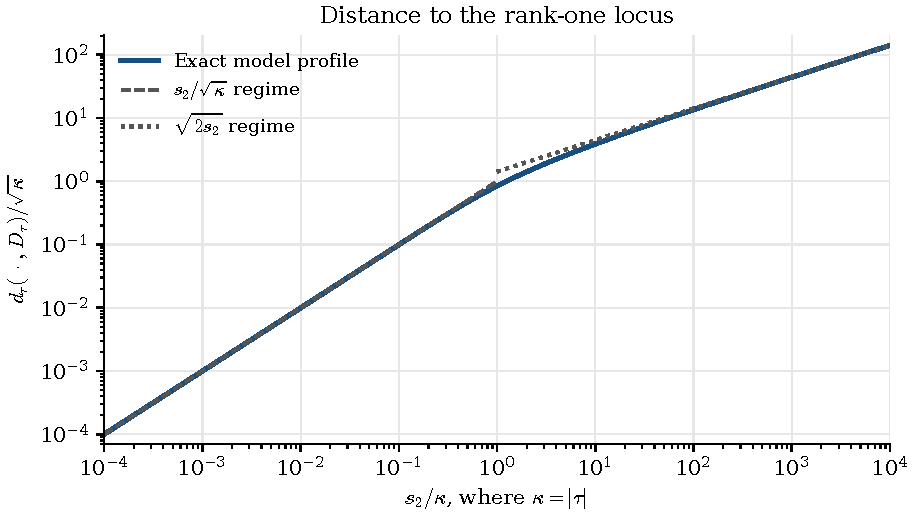
\includegraphics[width=.94\textwidth]{figures/distance-profile.pdf}
\caption{The exact model distance to $D_\tau$, divided by
$\sqrt{\kappa}$, as a function of $s_2/\kappa$, where
$\kappa=|\tau|$. The two reference lines show the limiting regimes.
The actual moduli distance has this profile with the relative error
in Theorem~\ref{thm:distances}. The plotted curve is evaluated from
\eqref{eq:profile-intro}; it is not an empirical fit.}
\label{fig:distance}
\end{figure}

\begin{lemma}\label{lem:short-paths}
The radius $r_\tau$ is 1-Lipschitz. There is an absolute $L$ such
that any $p,q$ of radius at most $\rho$ can be joined inside
$\{r_\tau\le\rho\}$ with length at most $L\rho$.
\end{lemma}

\begin{proof}
The Euclidean radius is compact-invariant and 1-Lipschitz; subtracting
a compact vertical vector leaves its differential unchanged. This
proves the quotient assertion. For $\tau>0$, write
$A=U(\tau I+Q)^{1/2}$, $Q=BB^*$, and shrink
$B$ to $uB$, replacing $A$ by $U(\tau I+u^2Q)^{1/2}$.
The squared speed is
\[
\tr Q+\tr\bigl(u^2Q^2(\tau I+u^2Q)^{-1}\bigr)\le2\tr Q.
\]
The cost is at most $r_\tau$ and radius decreases. The two resulting
points on the zero section can be joined at cost $D\sqrt\tau$, where
$D$ is the diameter of the fixed Grassmannian quotient metric.
Since $r_\tau^2\ge2\tau$, $L=2+D/\sqrt2$ works. The negative
case is symmetric. At zero join both points radially to the vertex,
at total cost at most $2\rho$.
\end{proof}

\subsection{Fibre metrics and comparison with the wall}

The zero-section metric is $\kappa$ times its Stiefel quotient metric.
For a rank-one matrix $N=suv^*$, with $s>0$ and orthogonal unit
$u,v$, put $W=(u,v)^\perp\simeq\CC^3$. For $\tau>0$ a point in
its $\PP(W)$ fibre has representative
\[
A=(\sqrt p\,u,\sqrt\tau\,w),\qquad
B=\begin{pmatrix}\sqrt q\,v^*\\0\end{pmatrix},\qquad
\|w\|=1,\quad p,q>0,\quad p-q=\tau,\ pq=s^2.
\]
A Hopf-horizontal variation $\dot w\perp w$ in $W$ has sole
variation $\dot A_2=\sqrt\tau\,\dot w$. Every complex orbit variation
has $A$-columns in $\langle u,w\rangle$, so this tangent is
orthogonal to the whole complex vertical space. The induced fibre
metric is exactly $\tau g_{\rm FS}$, where $g_{\rm FS}$ is the
unit-sphere Hopf quotient metric. This is independent of $s$.
Adjoint interchange gives the negative case with factor $\kappa$.

\begin{lemma}\label{lem:outer-model}
On the common rank-two locus of $M_\tau$ and $M_0$, identified by $N$,
\begin{equation}\label{eq:outer-model}
e^{-\arsinh(|\tau|/(2s_2))}g_0^{\rm q}
\le g_\tau^{\rm q}\le
e^{\arsinh(|\tau|/(2s_2))}g_0^{\rm q}.
\end{equation}
\end{lemma}

\begin{proof}
Choose a zero-level representative
$A_0=U\diag(\sqrt{s_1},\sqrt{s_2})$,
$B_0=\diag(\sqrt{s_1},\sqrt{s_2})V^*$.
Its representative at level $\tau$ in the same complex orbit is
$(A_0e^S,e^{-S}B_0)$, with
\begin{equation}\label{eq:outer-S}
S=\diag(\lambda_1,\lambda_2),\qquad
\lambda_i=\tfrac12\arsinh\bigl(\tau/(2s_i)\bigr).
\end{equation}
This solves $2s_i\sinh(2\lambda_i)=\tau$ and preserves $AB$.
Hermitian functional calculus defines $S$ smoothly even at a repeated
positive singular value.

On a central real moment level inside the complex equation, the quotient
metric is also the infimum over the full \emph{complex} orbit tangent.
Indeed the imaginary compact-orbit directions are the gradients of
the real moment components, hence are normal to the level.
Compact vertical directions are orthogonal to them because the moment
value is central. Their joint orthogonal complement is exactly the
compact horizontal tangent.

Differentiating the point-dependent gauge in~\eqref{eq:outer-S}
adds a complex vertical vector to its linear action on a tangent.
This is true without commutativity of $S$ and its derivative: the
logarithmic derivative of $e^S$ is a Lie algebra element. The added
vector vanishes in the complex vertical infimum. The linear action
transports the vertical space and changes squared ambient norms by
factors between $e^{-2\|S\|}$ and $e^{2\|S\|}$. Since
$2\|S\|=\arsinh(|\tau|/(2s_2))$, this proves the result.
\end{proof}

The error in~\eqref{eq:outer-model} is $O(|\tau|/s_2)$ when that ratio
is small. Its loss at rank one is intentional: the complete inner
model and the exact distance profile describe the region where this
outer approximation is no longer small.
